% \ednote{FR: Picking 1 of the 3 queries given here is enough as an example.
% The paragraph 'Additional Examples' should be removed, and 1-2 of the difficult queries given there should be given as advanced examples.
% Try to give one screenshot of the result of a complex query. Say how many results the queries return.}

In this section, we evaluate the ULO framework, i.e. the ULO ontology and the generated RDF data by showing how they could be exploited using standard tools of the Semantic Web tool stack.

We have set up an instance of Virtuoso Open-Source Edition\footnote{\url{https://github.com/openlink/virtuoso-opensource}}, which reads the exports described in Section~\ref{sec:isabelle-export} and provides a web interface with a SPARQL endpoint to experiment with the ULO dataset.
Then we have tried several queries with promising results (just one shown below for lack of space).
The queries are not meant to be a scientific contribution per se: they just show how much can be accomplished with the ULO dataset with standard tools in one afternoon.

\paragraph{Example query: all recursive functions on $\mathbb{N}$} For this, we use the \lstinline|ulo:inductive-on| relation to determine inductive definitions on a type \lstinline|?y|, which we restrict to one that is aligned with the type \lstinline|nat_lit| of natural numbers from the interface theory \lstinline|NatLiterals| in the Math-in-the-Middle Ontology.
\begin{lstlisting}
SELECT ?x ?y WHERE {
  ?x ulo:inductive-on ?y .
  http://mathhub.info/MitM/Foundation?NatLiterals?nat_lit ulo:aligned-with ?y . }
\end{lstlisting}
Note that we use alignments~\cite{MueGauKal:cacfms17} with concepts from an interface theory as a way of specifying ``the natural numbers'' across theorem prover libraries. The result is a list of pairs: each pair combines a specific implementation of natural numbers (Isabelle has several, depending on the object-logic), together with a function defined by reduction on it. A subset of the results of this query are shown in Figure~\ref{fig:query}.

\begin{figure}[t]\centering
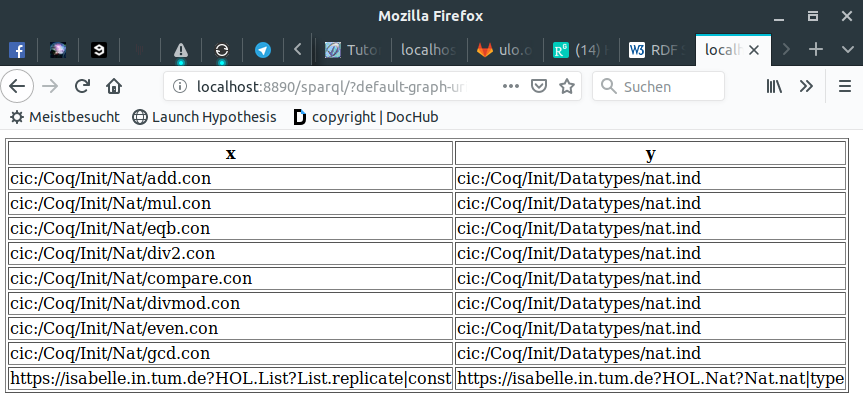
\includegraphics[width=\textwidth]{ulo_queryresult}
\caption{Virtuoso Output for the Example Query using Alignments}\label{fig:query}
\end{figure}

\ednote{check if Dennis can supply Isabelle screenshots}

%Similarly,  we can e.g. use the \lstinline|ulo:orcid| and \lstinline|dcterms:creator| properties to e.g. query for all theorems by Michael Kohlhase or Claudio Sacerdoti Coen using their ORCID.

\paragraph{Transitive Queries} The result of the query above only depends on the explicitly generated RDF triples. Semantic Web tools that understand OWL allow more complex queries. % For example, if we want to query for \emph{all theorems whose proofs depend on statements with incomplete proofs}, it is sufficient to specify in the ontology that \ind{uses} is transitive, and add a property to identify incomplete proofs.
For example, Virtuoso implements custom extensions that allow for querying the transitive closure of a relation. The resulting query syntax is a little convoluted, and we omit some details in the example below.
\begin{lstlisting}
SELECT ?o ?dist WHERE { {
      SELECT ?s ?o WHERE { ?s ulo:uses ?o }
    }
    OPTION ( TRANSITIVE, t_distinct, t_in(?s), t_out(?o), t_min (1),
             t_max (10), t_step ('step_no') as ?dist ) .
    FILTER ( ?s = <cic:/Bignums/BigN/BigN/BigNring.con> )
  }
ORDER BY ?dist DESC 2
\end{lstlisting}
The above code queries for all symbols recursively used in the (effectively randomly chosen) Lemma \texttt{BigNring} stating that the ring of arbitrary large natural numbers in base $2^{31}$ is a semiring; the output for that query is shown in Figure \ref{fig:query2}.


\begin{figure}[ht]\centering
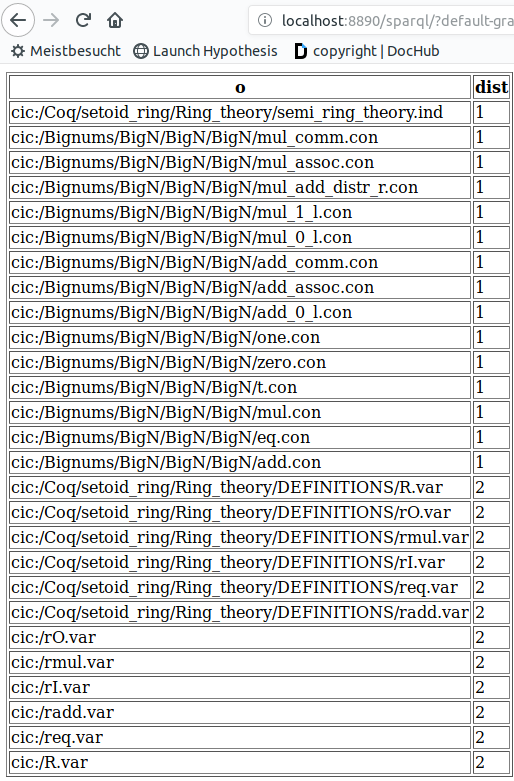
\includegraphics[width=0.5\textwidth]{ulo_queryresult2}
\caption{Virtuoso Output for the Transitive Example Query}\label{fig:query2}
\end{figure}

%then we have to use that the \ind{ulo:uses} is transitive.
%This is specified in the OLW2 implementation ULO ontology and can be used by sufficiently powerful tools (e.g. Virtuoso).
%Given that Virtuoso implicitly computes the transtive closure we can answer the query using a very similar query as the one above (given an alignment for proof gap objects).

Interesting examples of library management queries which can be modeled in SPARQL (and its various extensions, e.g. by rules) are found in~\cite{conf/lpar/AspinallDL12}. Instead~\cite{AGSTZ:ContMathSearchWhelp04,MKM04:AspertiS04} show examples of interesting queries (approximate search of formulae up to instantiation or generalization) that can be implemented over RDF triples, but that requires an extension of SPARQL with subset and superset predicates over sets.
% \ednote{DM: Add detailed examples (transitivity?)}
%\begin{center}
%\begin{tabular}{|c|c|}\hline
%	\lstinline|x| & \lstinline|y| \\\hline\hline
%	\tiny\lstinline>https://isabelle.in.tum.de?HOL.List?List.replicate|const> & \tiny\lstinline>https://isabelle.in.tum.de?HOL.Nat?Nat.nat|type> \\\hline
%	\tiny\lstinline|cic:/Coq/Init/Nat/add.con| & \tiny\lstinline|cic:/Coq/Init/Datatypes/nat.ind| \\\hline
%	\tiny\lstinline|cic:/Coq/Init/Nat/mul.con| & \tiny\lstinline|cic:/Coq/Init/Datatypes/nat.ind| \\\hline
%	\tiny\lstinline|cic:/Coq/Init/Nat/div2.con| & \tiny\lstinline|cic:/Coq/Init/Datatypes/nat.ind| \\\hline
%\end{tabular}
%\end{center}
%
%\paragraph{All theorems by Michael Kohlhase or Claudio Sacerdoti Coen}\ 
%\begin{lstlisting}
%SELECT ?x WHERE {
% ?x [ulo:theorem ?y ; dcterms:creator ?z]
% {?z ulo:orcid "0000-0002-4360-6016"} 
%   UNION
% {?z ulo:orcid "0000-0002-9859-6337"} }
%\end{lstlisting}
%
%\paragraph{All theorems with incomplete Proofs}\
%\begin{lstlisting}
%SELECT ?x WHERE {
%  ?x [ulo:proof ?y ; ulo:uses ?z]
%  ?z ulo:aligned-with http://mathhub.info/MitM?proofs?gap
%  OPTION ( TRANSITIVE, t_distinct, t_in(?x),t_out(?z)) }
%\end{lstlisting}
%This query is similar to the one about all inductive functions above, only that we use transitivity for the \lstinline|ulo:uses| relation (SPARQL syntax simplified).\ednote{MK: I have copied this by pattern matching from \url{https://virtuoso.openlinksw.com/tutorials/sparql/SPARQL_Tutorials_Part_5/SPARQL_Tutorials_Part_5.html} without understanding much.\\DM: Doing this properly gets ugly and elaborate; I would leave it simplified.}
%
%\paragraph{Additional examples} include
%\begin{itemize}
%\item Authors with the slowest proofs (in verification)
%\item Libraries ordered by dependency and check-time
%\item Dependency paths by cumulative check time
%\item Subgraphs by Topology; e.g. all situations of the form
%  \begin{tikzpicture}[baseline=(c.base),xscale=1.4,yscale=.8]
%    \node (lo) at (0,1) {$\bullet$};
%    \node (ro) at (1,1) {$\bullet$};
%    \node (lu) at (0,0) {$\bullet$};
%    \node (ru) at (1,0) {$\bullet$};
%    \node (c) at (.5,.5){};
%    \draw[include] (lu) -- (lo) ;
%    \draw[include] (ru) -- (ro);
%    \draw[struct] (lo) -- node[above]{\tiny deps} (ro);
%  \end{tikzpicture}
%  in a given library.
%\end{itemize}
%%% Local Variables:
%%% mode: latex
%%% mode: visual-line
%%% fill-column: 5000
%%% TeX-master: "report"
%%% End:

%  LocalWords:  ednote mathbb MueGauKal:cacfms17 centering includegraphics textwidth queryresult emph hline texttt BigNring AGSTZ:ContMathSearchWhelp04,MKM04:AspertiS04 generalization
